\subsection{Understandability}



\begin{frame}
\frametitle{Imagetest}
\begin{figure}[h]
  \centering
  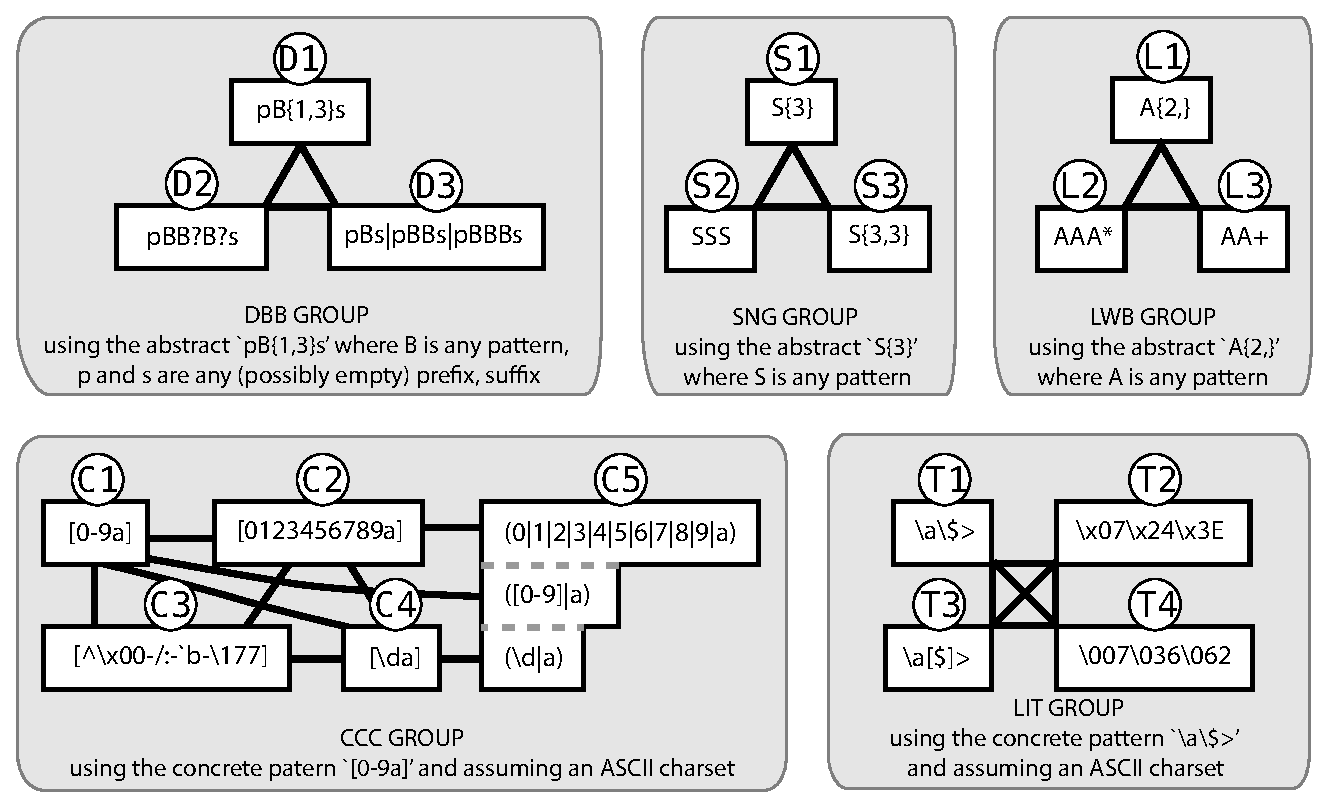
\includegraphics[scale=0.4]{nontex/illustrations/refactoringTree.eps}
  \caption{Equivalence classes with various representations of semantically equivalent representations within each class. DBB = Double-Bounded, SNG = Single Bounded, LWB = Lower Bounded, CCC = Custom Character Class and LIT = Literal}
  \label{fig:refactoringTree}
\end{figure}
\end{frame}
\note[itemize]{
    \item pt 1
    \item pt 2
}

